\documentclass{beamer}
\usetheme{Boadilla}
\usepackage{hyperref}
\usepackage{graphicx}
\usepackage{multimedia}
\usepackage{fancyvrb}
\usepackage{multicol}
\usepackage{adjustbox}
\usepackage{tikz}
\usetikzlibrary{shapes,positioning}
\newcommand{\foo}{\hspace{-2.3pt}$\bullet$ \hspace{5pt}}
\usepackage{subfig}
\usepackage[backend=biber,authordate]{biblatex-chicago}
\addbibresource{citations.bib}
\usepackage{pgfpages}
\usepackage{xcolor}
\definecolor{ao(english)}{rgb}{0.0, 0.5, 0.0}
\definecolor{burgundy}{rgb}{0.5, 0.0, 0.13}
%\setbeameroption{show notes}
\setbeameroption{show notes on second screen=right}
%\setbeameroption{hide notes}

\title{Pitch Tracking}
\author{Sevag Hanssian}
\date{March 23, 2021}
\institute{MUMT 621, Winter 2021}
\setbeamertemplate{navigation symbols}{}

\begin{document}

\begin{frame}
\maketitle
\end{frame}

\begin{frame}
	\frametitle{Pitch as a perceptual phenomenon}
	Pitch is the perceptual correlate of frequency, and the aspect of auditory sensation whose variation is associated with musical melodies.\footfullcite{plack}\\\ \\
	Pitch of a pure tone is its frequency; pitch of a complex tone is its lowest (or fundamental) frequency.\\\ \\
	Pitch can be quantified using fundamental frequency (or $\mathit{f0}$); interchangeable terms outside psychoacoustical studies.\footfullcite{crepe}
\end{frame}

\note{
	\begin{itemize}
		\item
			it's a bit more complicated. there's also a relationship between loudness and perceived pitch
			previous bad definition:  the attribute of auditory sensation in terms of which sounds may be ordered on a scale extending from low to high\\
			It requires the words ``low'' and ``high'' to be associated with pitch or frequency rather than with loudness or intensity, for example.
	\end{itemize}
}

\begin{frame}
	\frametitle{Pitch tracking algorithms}
	\begin{itemize}
		\item
			Candidate-generating function with pre- and post-processing to produce the pitch curve\footcite{crepe}
		\begin{itemize}
			\item
				Cepstrum 
			\item
				Autocorrelation function
			\item
				Average magnitude/square difference function (AMDF, ASDF)
			\item
				Normalized cross-correlation function (RAPT, PRAAT)
			\item
				Cumulative mean normalized difference (YIN)
		\end{itemize}
	\item
		SWIPE: template matching with spectrum of sawtooth waveform
	\item
		pYIN: probabilistic YIN with Hidden Markov Models (HMM) to decode most probably pitch sequences (best performing\footfullcite{comparison1}, \footfullcite{comparison2})
	\item
		WavePitch: based on the fast lifting wavelet transform (FLWT)
	\end{itemize}
\end{frame}

\note{
	\begin{itemize}
		\item
			YIN = yin and yang. the interplay of autocorrelation and cancellation
	\end{itemize}
}

\begin{frame}
	\frametitle{Autocorrelation}
	\begin{figure}
		\subfloat{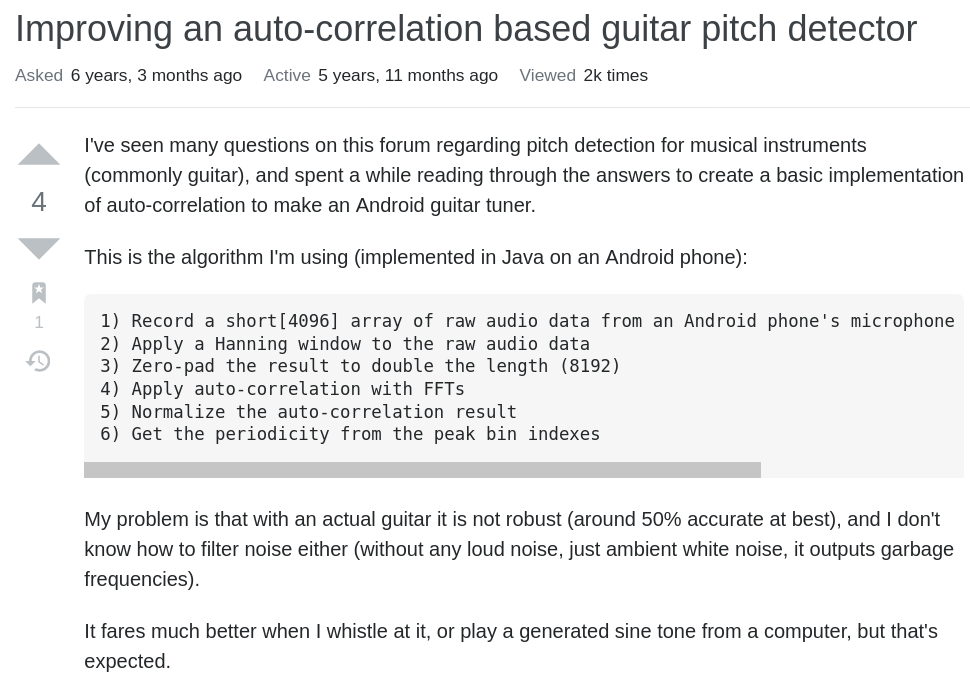
\includegraphics[width=5.8cm]{./dsp_q.png}}
		\hspace{0.1em}
		\subfloat{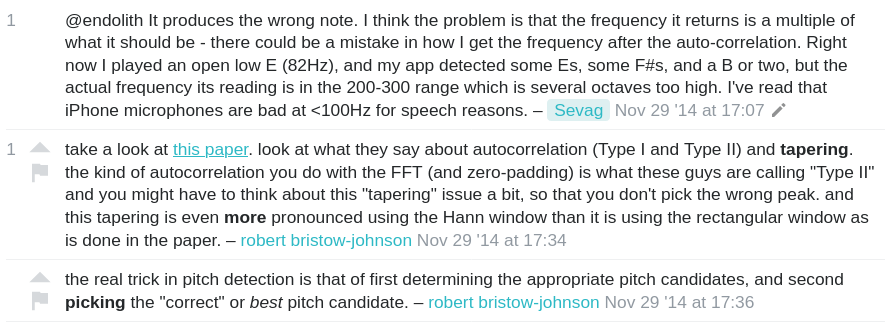
\includegraphics[width=5.8cm]{./dsp_q2.png}}
		\caption{Na{\"i}ve autocorrelation for guitar\footnote{\href{https://dsp.stackexchange.com/questions/19379/improving-an-auto-correlation-based-guitar-pitch-detector}{https://dsp.stackexchange.com/questions/19379/improving-an-auto-correlation-based-guitar-pitch-detector}}}
	\end{figure}
\end{frame}

\begin{frame}
	\frametitle{Autocorrelation}
	Autocorrelation: measure signal self-similarity by multiplying it with lagged copies of itself
	\begin{figure}
		\movie[width=8cm,height=5cm]{}{autocorrelation_example.gif}
		\caption{Animation of sine wave autocorrelation\footnote{http://qingkaikong.blogspot.com/2017/01/signal-processing-how-autocorrelation.html}}
		\vspace{-1em}
	\end{figure}
\end{frame}

\note{
	\begin{itemize}
		\item
			YIN = yin and yang. the interplay of autocorrelation and cancellation
	\end{itemize}
}

\begin{frame}
	\frametitle{Autocorrelation -- peak picking}
	Peak picking: measure signal periodicity by measuring inter-peak distance on autocorrelation
	\begin{figure}
		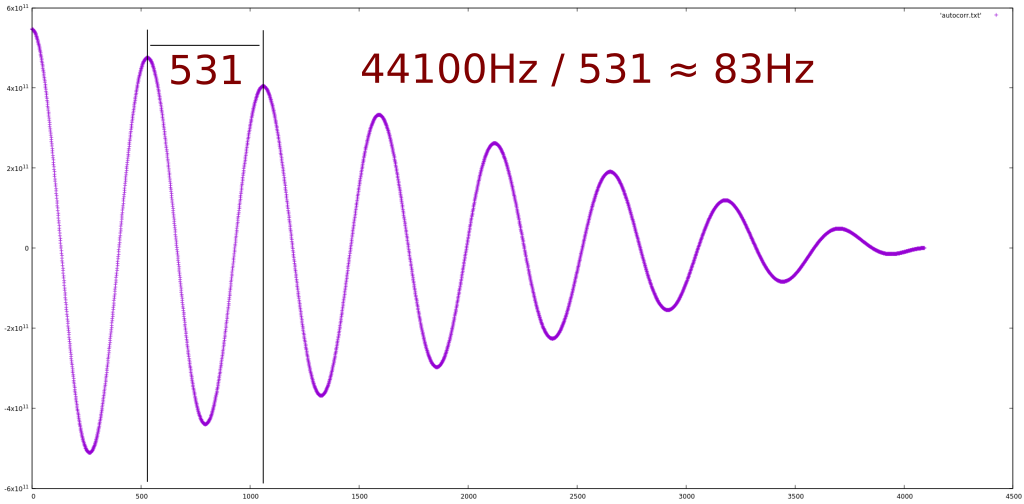
\includegraphics[width=7.5cm]{./sine_autocorrelation.png}
		\caption{Autocorrelation peaks, example: 83Hz sine wave\footnote{https://github.com/sevagh/pitch-detection/tree/master/misc/mcleod}}
	\vspace{-1em}
	\end{figure}
	Peaks: [529, 1060, 1591, 2122, 2652, 3181, 3702]\\
	Lag increment: \textasciitilde531 samples\\
	Convert lag to pitch: 44100 Hz (sample rate) divided by 531 gives \textasciitilde83Hz, which is the frequency of the sine wave.
\end{frame}

\begin{frame}
	\frametitle{YIN and McLeod Pitch Method -- better autocorrelation}
	\begin{figure}
		\subfloat[MPM's\footfullcite{mpm} normalized square difference function]{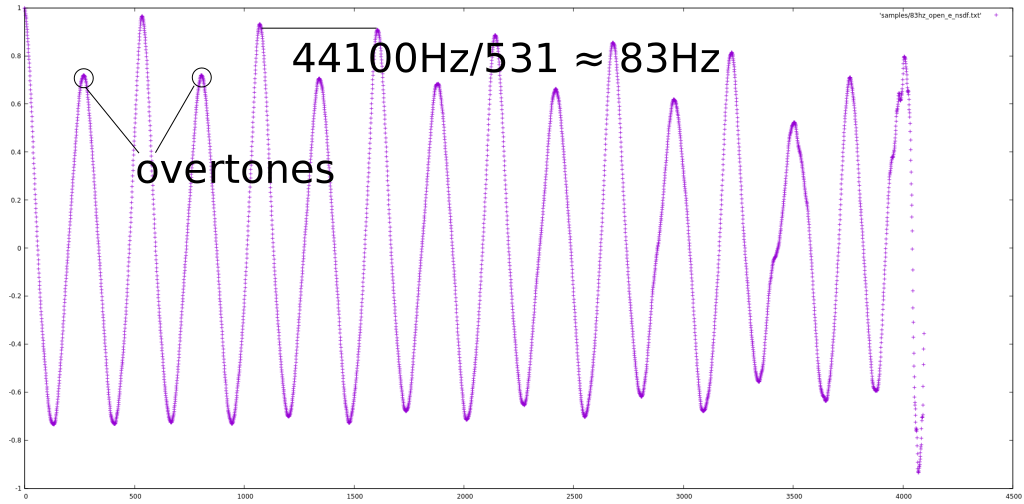
\includegraphics[width=5.75cm]{./open_e_nsdf.png}}
		\hspace{0.1em}
		\subfloat[YIN's\footfullcite{yin} cumulative mean normalized difference function]{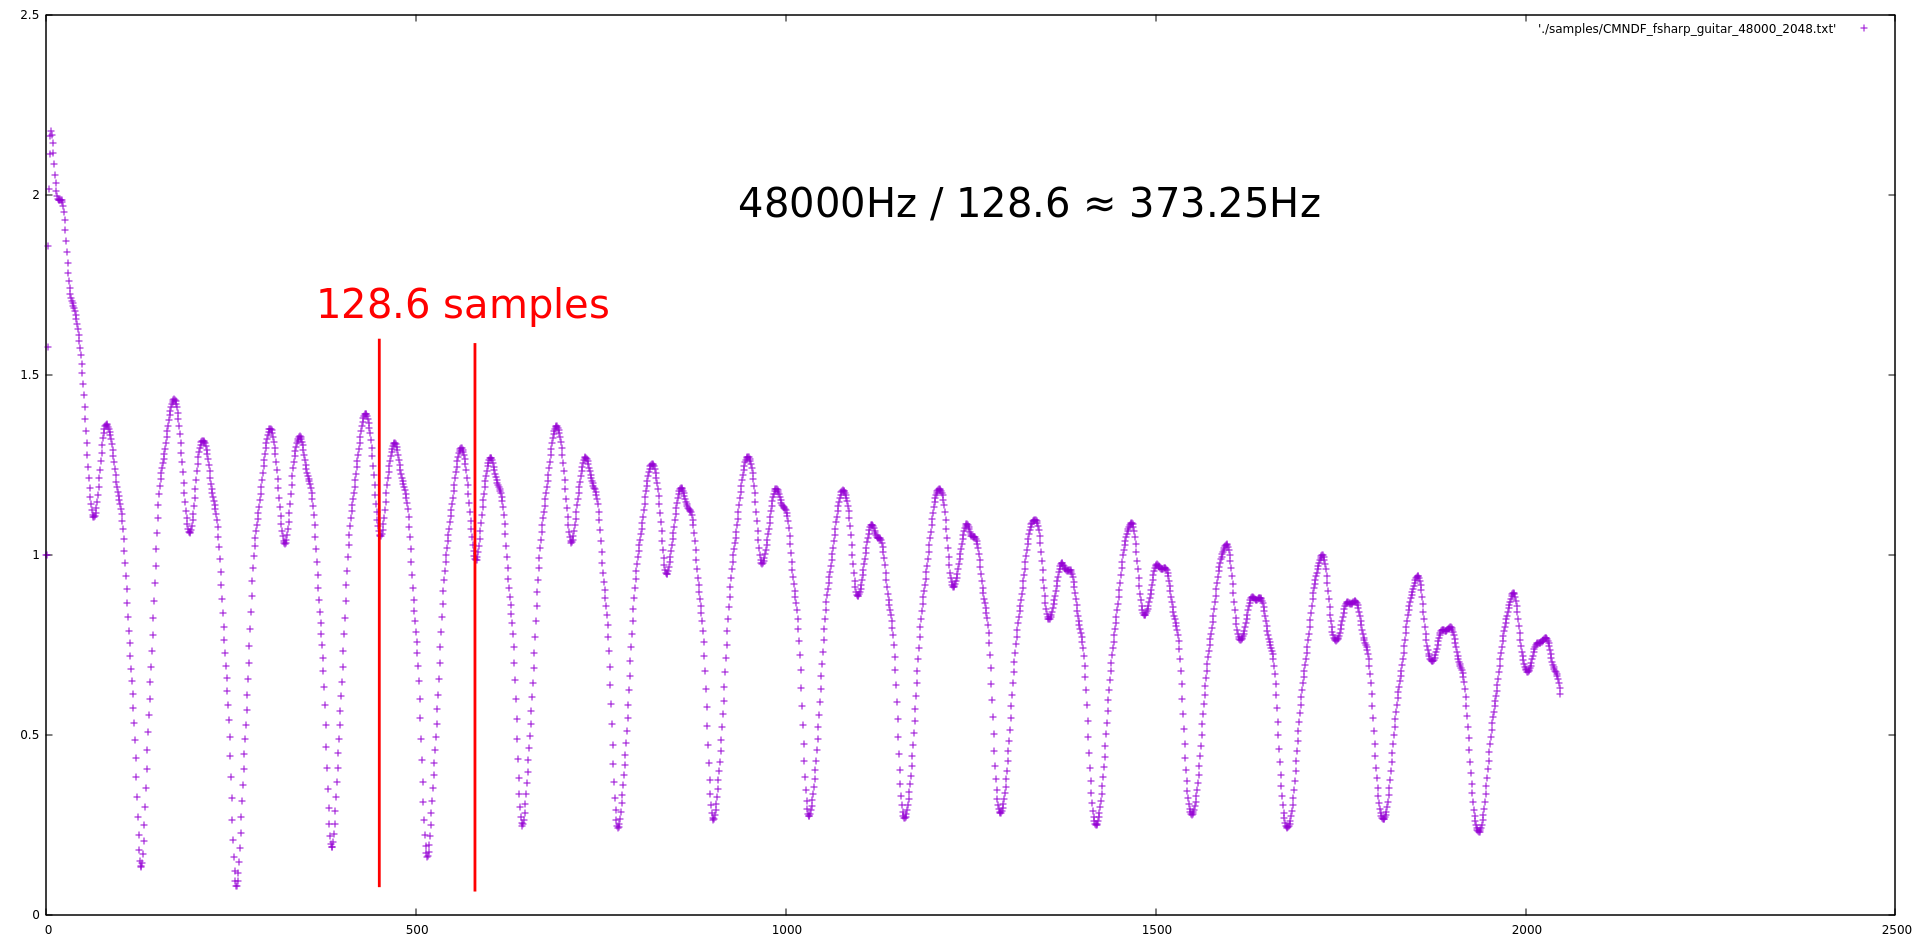
\includegraphics[width=5.75cm]{./cmndf.png}}
		\caption{YIN and MPM's variants of autocorrelation\footnote{https://github.com/sevagh/pitch-detection/tree/master/misc/mcleod, https://github.com/sevagh/pitch-detection/tree/master/misc/yin}}
	\end{figure}
\end{frame}

\note{
	\begin{itemize}
		\item
			Both functions related to autocorrelation, with the main correction that both discard the 0th lag -- signal max self-similarity at no lag.
	\end{itemize}
}

\begin{frame}
	\frametitle{YIN and McLeod Pitch Method -- better peak picking}
	Better peak picking: parabolic interpolation in both
	\begin{figure}
		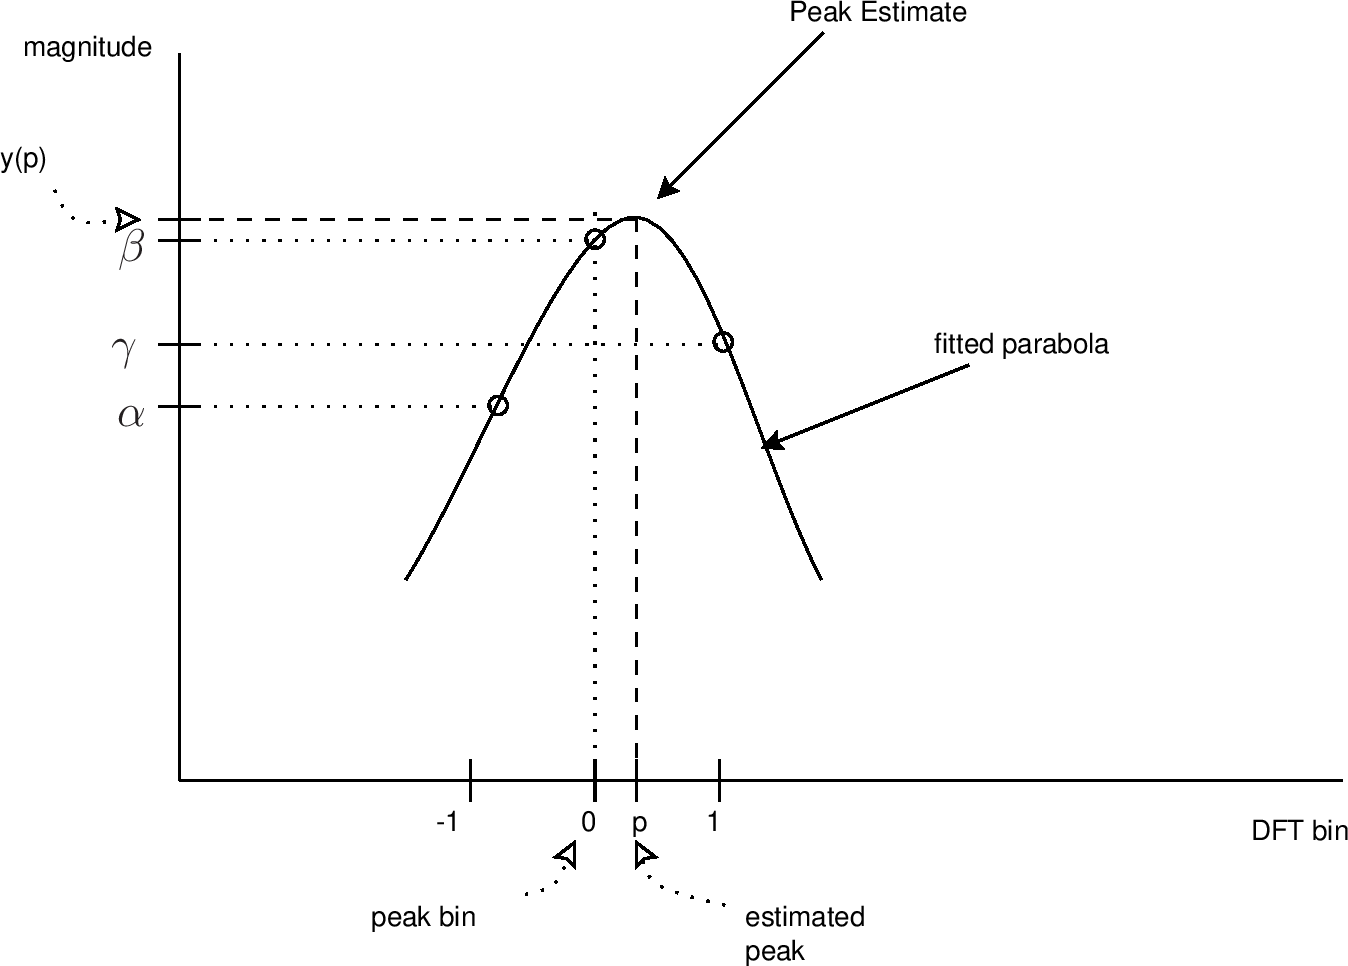
\includegraphics[height=6cm]{./parabolicinterp.png}
		\caption{Parabolic interpolation to improve peak picking\footnote{https://ccrma.stanford.edu/~jos/SpecAnal/Parabolic\_Interpolation.html}}
	\end{figure}
\end{frame}

\begin{frame}
	\frametitle{Autocorrelation vs. MPM}
	\begin{figure}
		\subfloat[Autocorrelation]{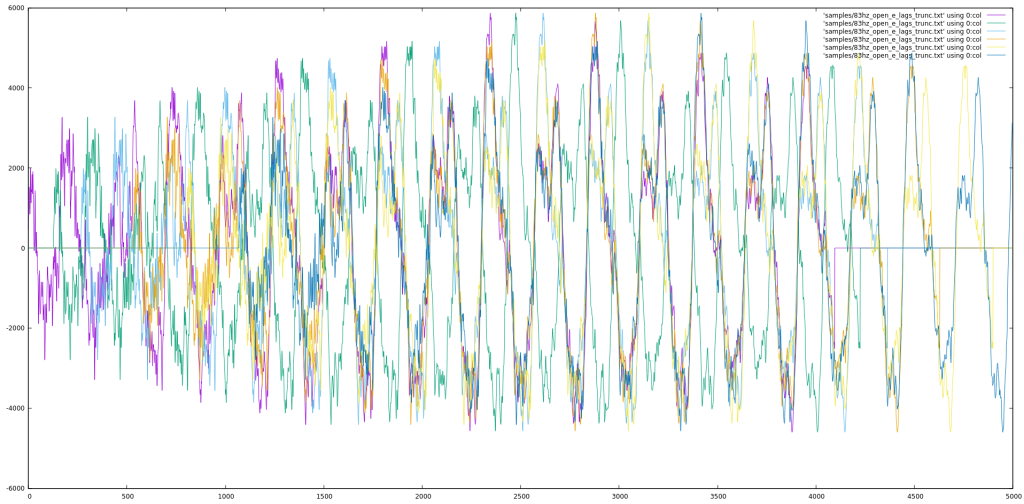
\includegraphics[width=5.75cm]{./open_e_peak_lags_wrong.png}}
		\hspace{0.1em}
		\subfloat[MPM]{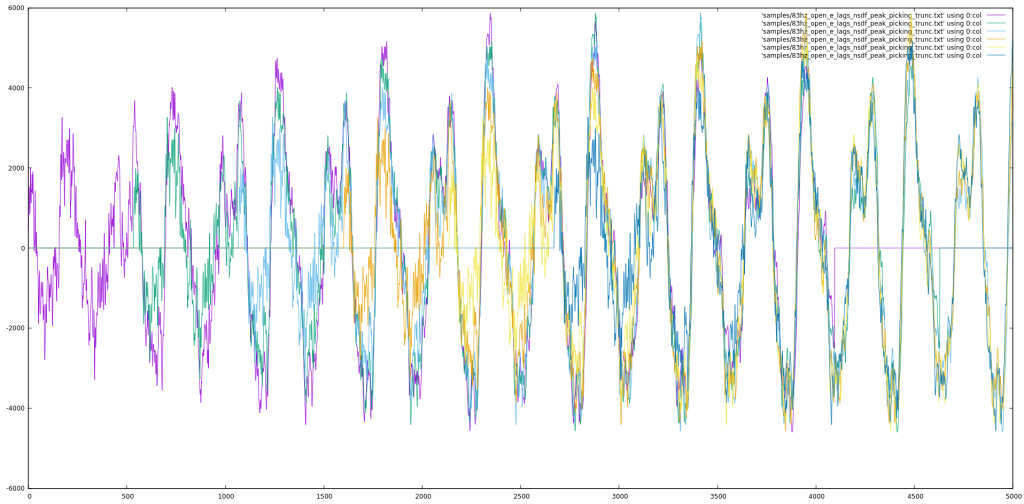
\includegraphics[width=5.75cm]{./open_e_nsdf_peak_lags_best.png}}
		\caption{Guitar signal superimposed on itself at peak lags\footnote{https://github.com/sevagh/pitch-detection/tree/master/misc/mcleod}}
	\end{figure}
\end{frame}

\begin{frame}
	\frametitle{Musical importance of pitch}
	Pitch is musically important to humans:\footfullcite{musicevo}
	\begin{itemize}
		\item
			Relationships between pitches (relative pitch) are more important than the absolute value. Sequence of pitch changes is the melodic contour
		\item
			Pitches separated by an octave have the same pitch chroma. Most (known) music depends on pitch relations defined by octaves
		\item
			Most (known) music in the world come from a discrete set of five to seven pitches arranged within an octave range
	\end{itemize}
\end{frame}

\note{
	\begin{itemize}
		\item
			Although rhythm is arguably just as important, if not more so, to many cultures' music, pitch has received far more attention in the literature we will review, likely due to its importance in Western music and the resultant theoretical ideas about how pitch functions in music.
		\item
			Pitch is universal, but the centrality of relative pitch indicates some innate auditory mechanism for encoding sound as pitch distances. Humans are good at ``melodic contour'', i.e. recognizing a melody whether it is transposed in tempo or octave.
		\item
			Limitations of memory and categorization, or sensory or computational bias to have intervals that approximate simple integer ratios
	\end{itemize}
}

\begin{frame}
	\frametitle{pYIN -- musically probable pitch sequences}
	\begin{figure}
		\subfloat[Multiple pitch candidates]{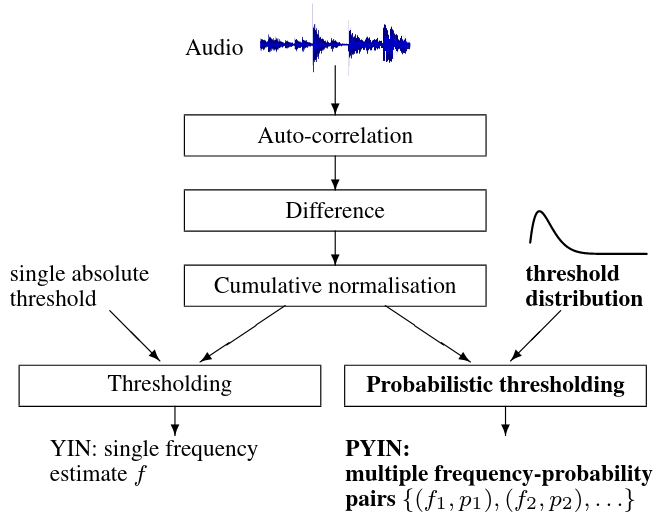
\includegraphics[height=3.5cm]{./pyin.png}}
		\hspace{0.1em}
		\subfloat[Pitch sequence HMM]{\makebox[0.4\textwidth]{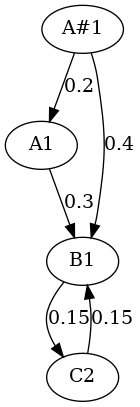
\includegraphics[height=3.5cm]{./pyin_hmm.png}}}
		\caption{Building probabilistic YIN\footfullcite{pyin} from YIN}
		\vspace{-1.5em}
	\end{figure}
	Pitch space is divided into 480 bins ranging over four octaves from 55Hz (A1) to just under 880Hz (A5) in steps of 10 cents (0.1 semitones)
\end{frame}

\note{
	\begin{itemize}
	\item
		the pitch candidates are used as observation probabilities. the transition probabilities are used to come up with the final pitch estimate
	\end{itemize}
}

\begin{frame}
	\frametitle{CREPE -- current state-of-the-art}
	\begin{quote}
		Best performing techniques such as the pYIN algorithm, are based on a combination of DSP pipelines and heuristics. [...] we propose a data-driven pitch tracking algorithm, CREPE, which is based on a deep convolutional neural network that operates directly on the time-domain waveform.\footcite{crepe}
	\end{quote}
	\begin{figure}
		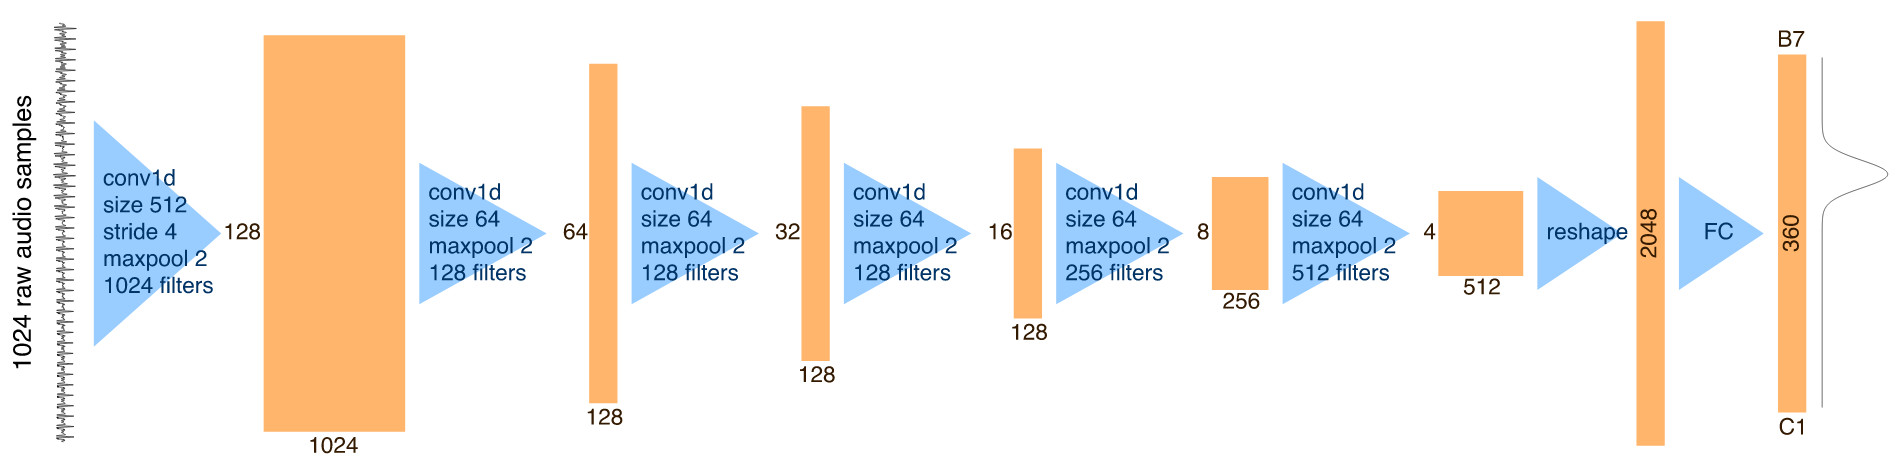
\includegraphics[width=10cm]{./crepe_arch.png}
		\caption{CREPE network architecture}
		\vspace{-1em}
	\end{figure}
	360 pitch values are are selected so that they cover six octaves with 20-cent intervals between C1 and B7, corresponding to 32.70 Hz and 1975.5 Hz.
\end{frame}

\begin{frame}
	\frametitle{Human pitch perception}
Initially two theories of human pitch perception: place and temporal.\footfullcite{moore}\\\ \\
	In the place theory (place coding), spectral analysis is done in the cochlea, so that the \textit{resolved} harmonics of a sound excite different parts of the basilar membrane (BM), firing neurons with different characteristic frequency.\\\ \\
	In the temporal theory (temporal coding, phase locking), the \textit{unresolved} harmonics form a complex waveform in the BM, and firing neurons lock to the phase of the envelope of the complex waveform.
\end{frame}

\note{
	\begin{itemize}
		\item
			First part is related to the tonotopic organization of the inner ear -- well established and independently confirmed in different studies. 100,200,300hz example. Second is still a matter of dispute
		\item
			gabor tf uncertainty principle. Our real sensitivity to <1\% differences in fundamental frequencies for resolved harmonics is better than what would be possible with firing rate/place coding, suggesting temporal coding
		\item
			More sophisticated models (which explain or account for human experimental data) require both place and temporal analyses (pitch can be recognized even with unresolved harmonics). Tentative neural component, processed after the ears -- two harmonics presented to different ears create the correct fundamental.
	\end{itemize}
}

\end{document}
